% Created 2024-03-04 Mon 08:28
% Intended LaTeX compiler: lualatex
\documentclass[bigger]{beamer}
\usepackage{amsmath}
\usepackage{fontspec}
\usepackage{graphicx}
\usepackage{longtable}
\usepackage{wrapfig}
\usepackage{rotating}
\usepackage[normalem]{ulem}
\usepackage{capt-of}
\usepackage{hyperref}
\usetheme[progressbar=foot, sectionpage=none, numbering=fraction]{metropolis}
\usepackage{tikz}
\usepackage{booktabs}
\usepackage{adjustbox}
\usepackage{diagbox}
\usepackage{latexcolors}
\usetikzlibrary{automata, positioning, arrows, arrows.meta}
\usepackage{diagbox}
\usepackage{dsfont}
\usepackage{amsmath}
\usepackage{fontawesome5}
\usepackage[ruled]{algorithm2e}
\usepackage[absolute, overlay]{textpos}
\definecolor{RedBrown}{RGB}{192, 4, 4} \setbeamercolor{progress bar}{fg=RedBrown} \setbeamercolor{title separator}{fg=RedBrown}
\setbeamercolor{progress bar in head/foot}{fg=RedBrown} \setbeamercolor{progress bar in section page}{fg=RedBrown} \setbeamercolor{alerted text}{fg=RedBrown}
\pretocmd{\tableofcontents}{\thispagestyle{empty}}{}{}
\addtocounter{framenumber}{-1}
\usepackage{listings}
\usepackage{xcolor}
\definecolor{codegreen}{rgb}{0,0.6,0}
\definecolor{codegray}{rgb}{0.5,0.5,0.5}
\definecolor{codepurple}{rgb}{0.58,0,0.82}
\definecolor{backcolour}{HTML}{f0f0f0}
\lstdefinestyle{mystyle}{
backgroundcolor=\color{backcolour},
commentstyle=\color{codegreen},
keywordstyle=\color{magenta},
numberstyle=\tiny\color{codegray},
stringstyle=\color{codepurple},
basicstyle=\ttfamily,
breakatwhitespace=false,
breaklines=true,
captionpos=b,
keepspaces=true,
numbers=none,
numbersep=5pt,
showspaces=false,
showstringspaces=false,
showtabs=false,
tabsize=2
}
\lstset{style=mystyle}
\usetheme{default}
\author{Andrea Pierré}
\date{March 4\textsuperscript{th}, 2024}
\title{Joint meeting}
\institute{Brown University}
\titlegraphic{\hfill
\includegraphics[height=1.5cm]{img/Brown Logo_2016_2 Color Process ST_1300.png}}
\setbeamercovered{transparent=10}
\setbeamertemplate{section in toc}[sections numbered]
\AtBeginSection[]{\begin{frame}[plain, noframenumbering]{Outline}    \setbeamertemplate{section in toc}[sections numbered]\setbeamertemplate{subsection in toc}[subsections numbered]\vspace{-0.8em}\tableofcontents[currentsection, currentsubsection]\end{frame}}
\AtBeginSubsection[]{\begin{frame}[plain, noframenumbering]{Outline}\setbeamertemplate{section in toc}[sections numbered]\setbeamertemplate{subsection in toc}[subsections numbered]\tableofcontents[currentsection,currentsubsection]\end{frame}}
\hypersetup{
 pdfauthor={Andrea Pierré},
 pdftitle={Joint meeting},
 pdfkeywords={},
 pdfsubject={},
 pdfcreator={Emacs 29.2 (Org mode 9.7)}, 
 pdflang={English}}
\begin{document}

\maketitle
\begin{frame}[plain]{Outline}
\tableofcontents
\end{frame}

\section{Online Deep RL training}
\label{sec:org99fed52}
\begin{frame}[label={sec:org692078c}]{Rewards \& steps}
\begin{center}
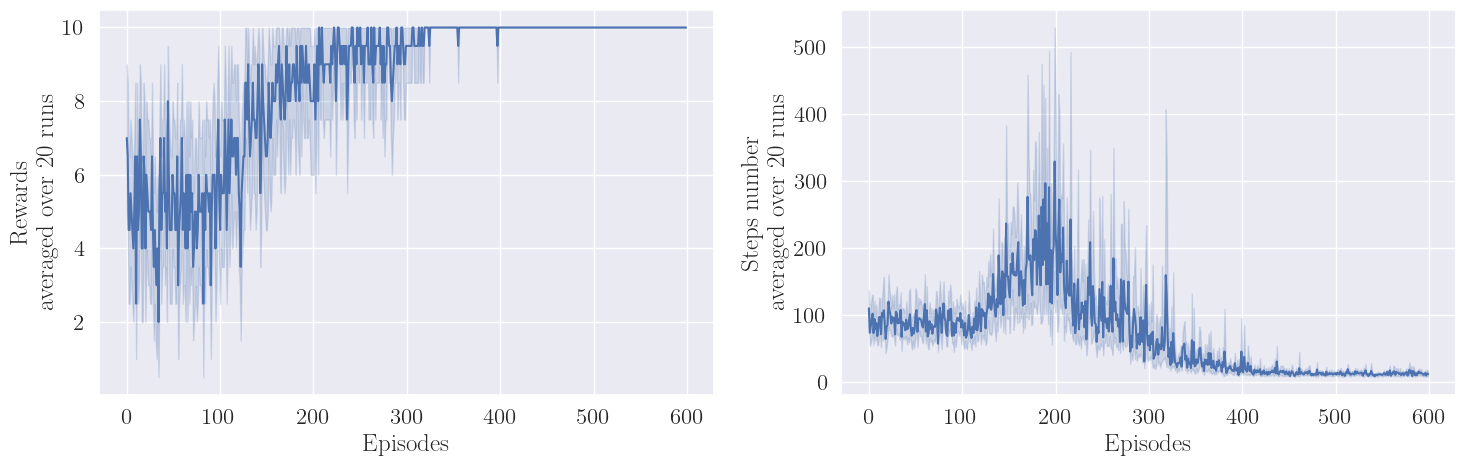
\includegraphics[width=\linewidth]{img/steps-and-rewards.png}
\end{center}
\end{frame}
\begin{frame}[<+->][label={sec:org86bc518}]{Why is it converging now?}
\begin{itemize}
\item Lights cues in the state?
\item Start training once replay buffer is full (5000 transitions) instead of when there are enough transitions for a batch (32 transitions)
\item Soft update of the networks weights (instead of sharp transition)
\item Huber loss instead of mean squared error \(\to\) should be less sensible to outliers
\item \alert{Remove ReLU on output layer!}
\end{itemize}
\end{frame}
\begin{frame}[label={sec:orgcf6bc7d}]{Loss, rewards \& steps distributions, exploration/exploitation rate}
\begin{center}
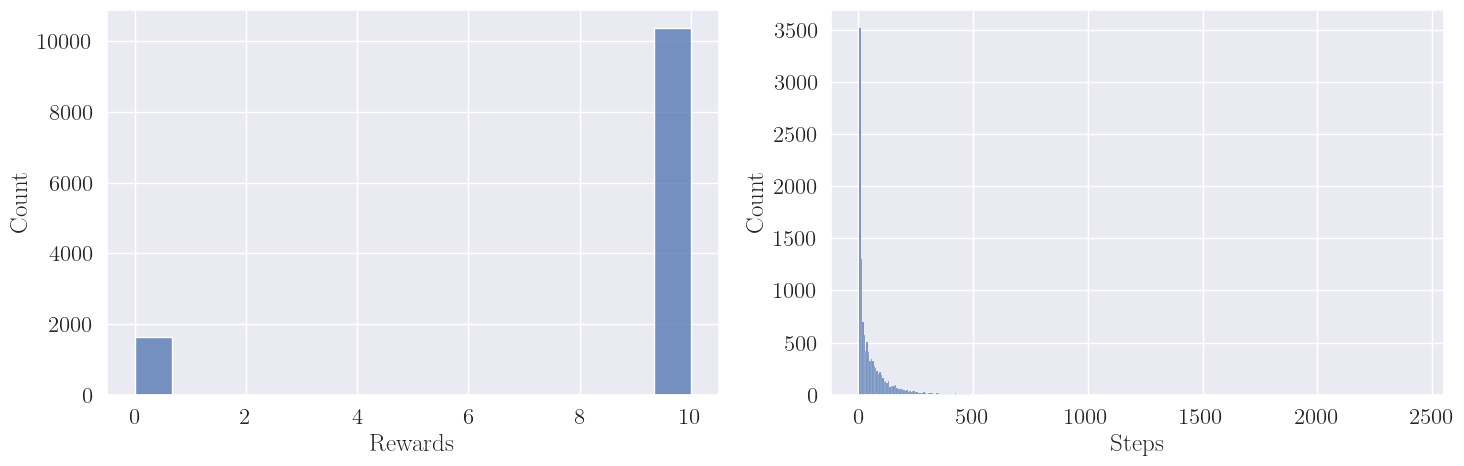
\includegraphics[width=.9\linewidth]{img/steps-and-rewards-distrib.png}
\end{center}
\begin{columns}
\begin{column}{0.4\columnwidth}
\begin{center}
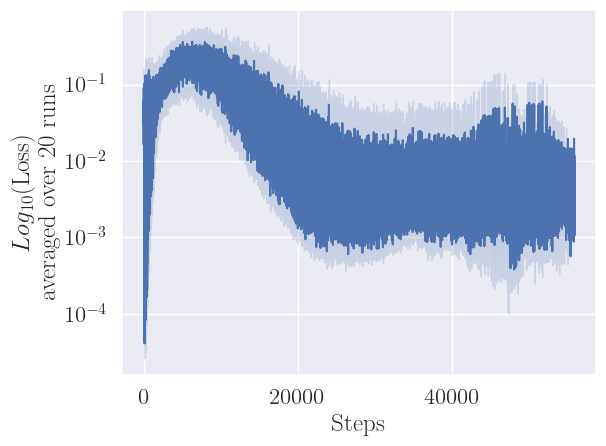
\includegraphics[width=.9\linewidth]{img/loss.png}
\end{center}
\end{column}
\begin{column}{0.4\columnwidth}
\begin{center}
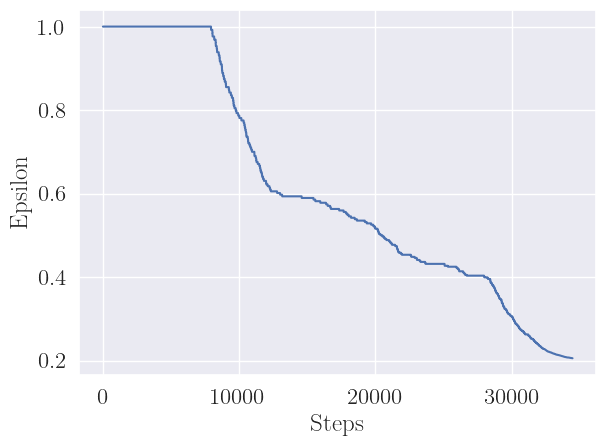
\includegraphics[width=.9\linewidth]{img/exploration-rate.png}
\end{center}
\end{column}
\end{columns}
\end{frame}
\begin{frame}[label={sec:org94fa2b4}]{Policy learned}
\begin{center}
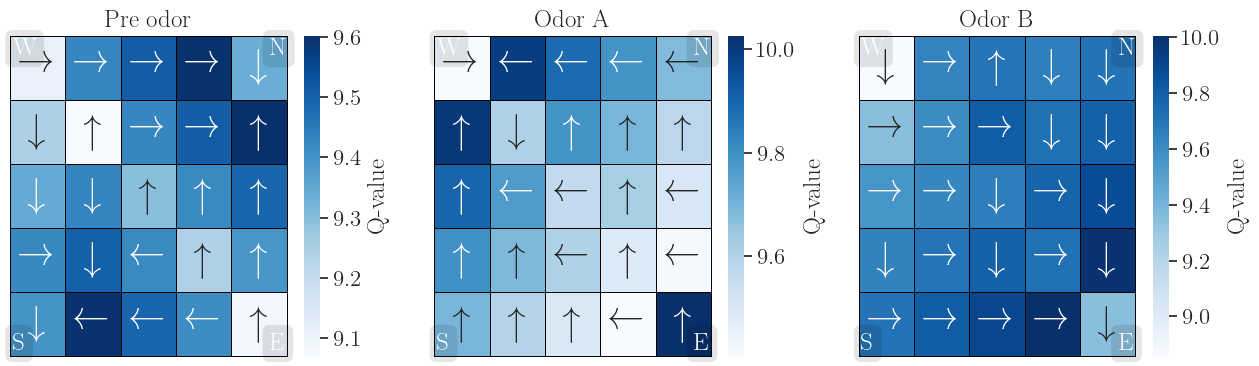
\includegraphics[width=\linewidth]{img/policy.png}
\end{center}
\end{frame}
\section{Generalization experiment}
\label{sec:orga723019}
\begin{frame}[label={sec:org237acba}]{Training only on the lower triangle}
\begin{center}
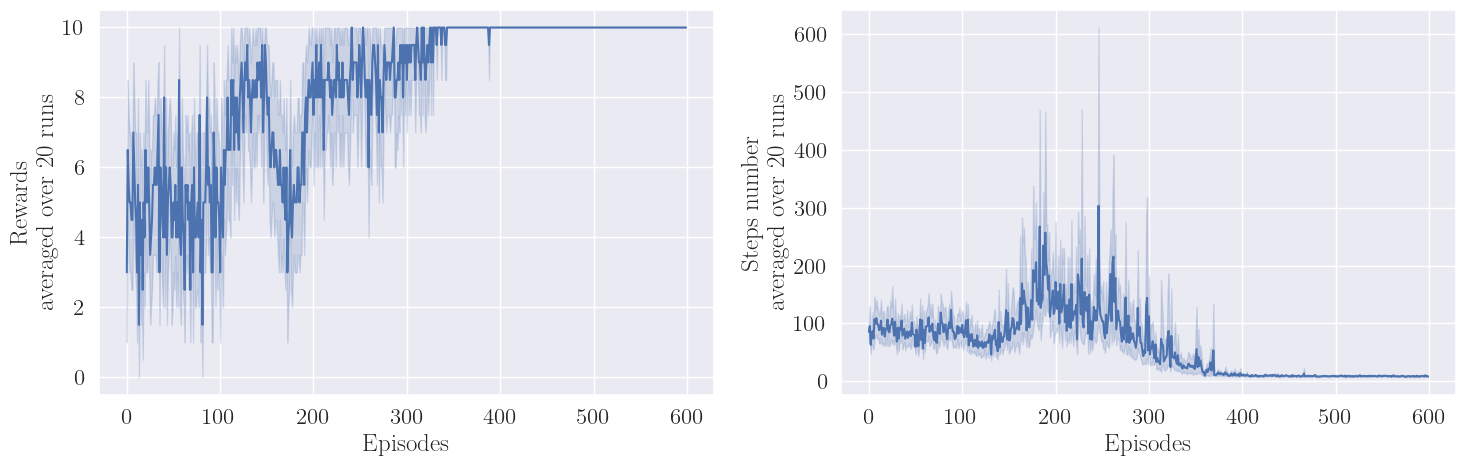
\includegraphics[width=\linewidth]{img/steps-and-rewards-lower-only.png}
\end{center}
\end{frame}
\begin{frame}[label={sec:org07aaa32}]{Generalization test: training only on the lower triangle then switch to upper triangle}
\begin{center}
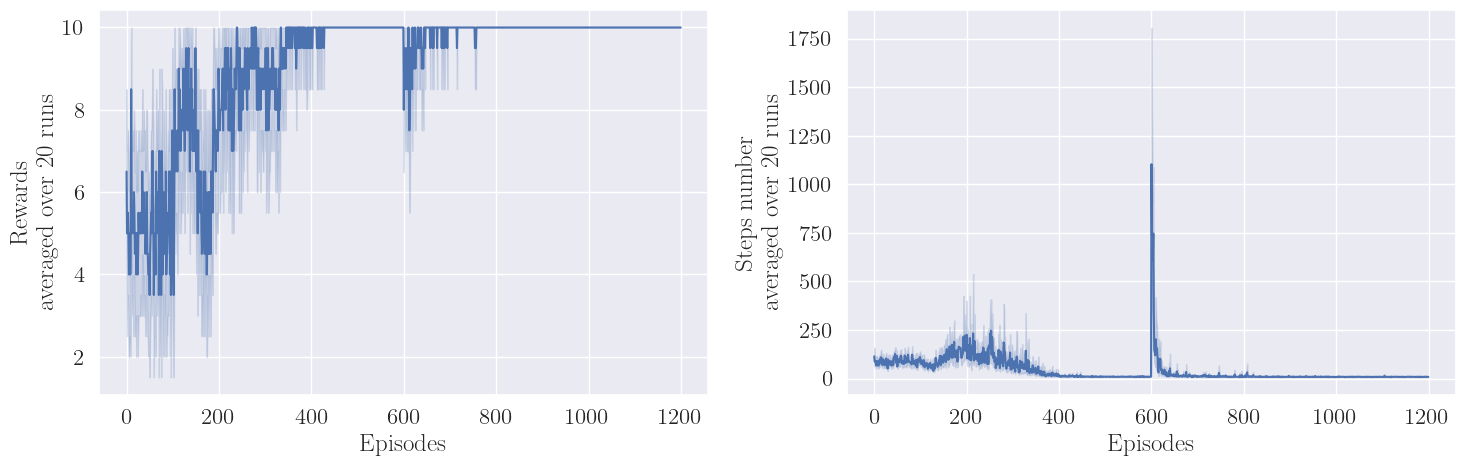
\includegraphics[width=.9\linewidth]{img/steps-and-rewards_upper-then-lower1.png}
\end{center}
\begin{center}
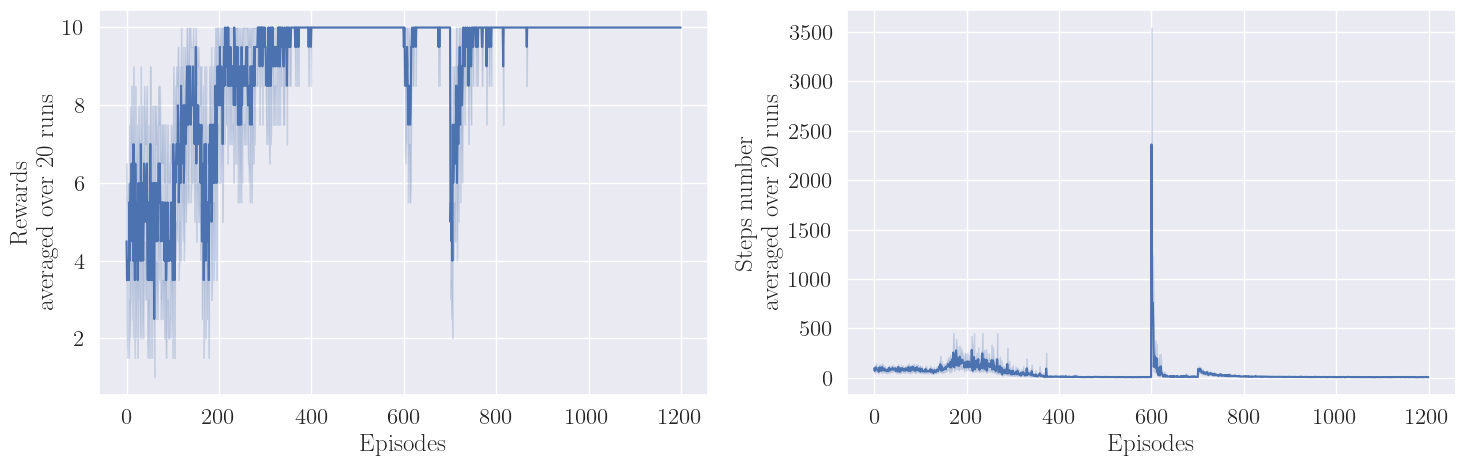
\includegraphics[width=.9\linewidth]{img/steps-and-rewards_upper-then-lower2.png}
\end{center}
\end{frame}
\begin{frame}[label={sec:org23cd4ca}]{Loss, exploration/exploitation rate}
\begin{columns}
\begin{column}{0.5\columnwidth}
\begin{center}
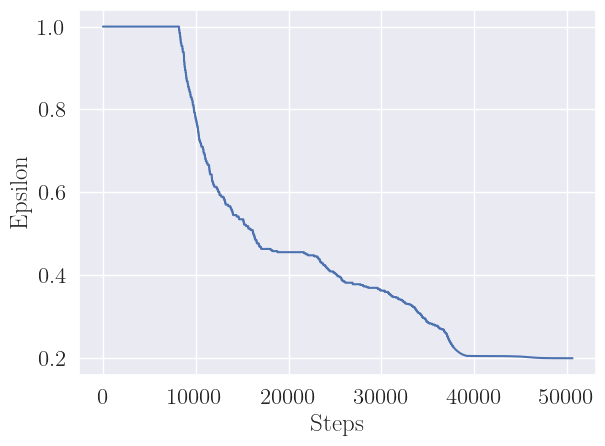
\includegraphics[width=.9\linewidth]{img/exploration-rate_upper-then-lower1.png}
\end{center}
\begin{center}
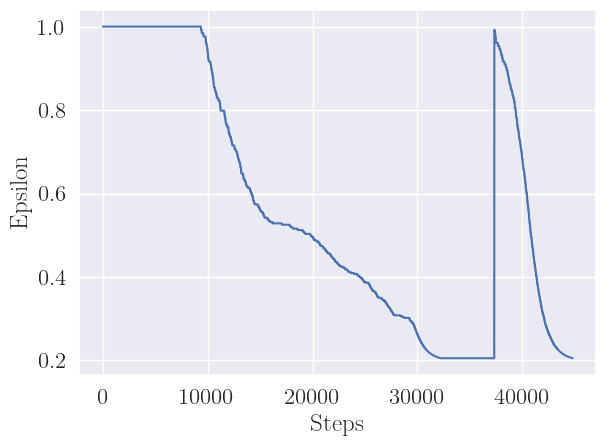
\includegraphics[width=.9\linewidth]{img/exploration-rate_upper-then-lower2.png}
\end{center}
\end{column}
\begin{column}{0.5\columnwidth}
\begin{center}
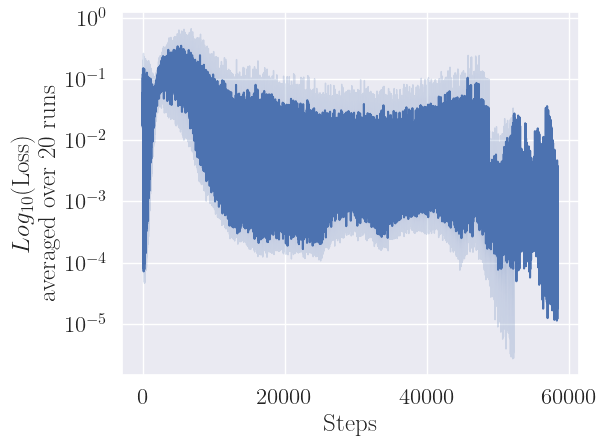
\includegraphics[width=.9\linewidth]{img/loss_upper-then-lower1.png}
\end{center}
\begin{center}
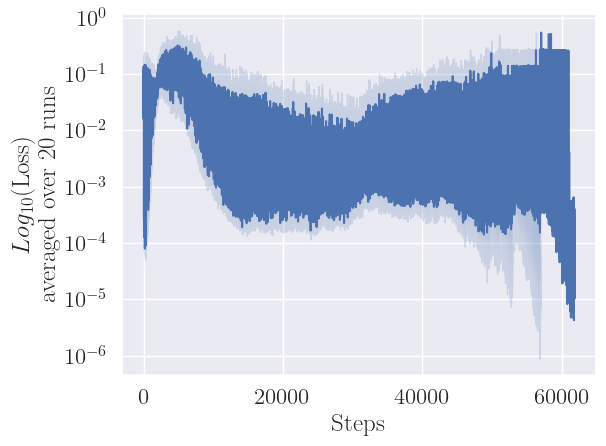
\includegraphics[width=.9\linewidth]{img/loss_upper-then-lower2.png}
\end{center}
\end{column}
\end{columns}
\end{frame}
\section{Discussion}
\label{sec:orgf6c4291}
\begin{frame}[<+->][label={sec:org2549330}]{Points of discussion}
\begin{itemize}
\item Debrief from the meeting with Thomas
\item Topics of discussion for future meetings?
\begin{itemize}
\item How to compare neural data with simulation data?
\item Journal club (e.g. MINDS paper, etc.)
\item Any other topics to add?
\end{itemize}
\end{itemize}
\end{frame}
\begin{frame}[label={sec:org7cf9124},standout]{~}
Thanks!
\end{frame}
\end{document}
